\chapter{Model Systemu}
\section{System zbiorników}
\indent Przedmiotem rozważań jest system 3 połączonych zbiornkiów. Zbiornik 3 służy jako rezerwuar wody. W zbiorniku 2 znajduje się koncentrat wykorzystywany do produkcji napoju. Oba te zbiorniki umieszczone są nad zbiornikiem 1, w którym woda miesza się z koncentratem tworząc gotowy produkt. Pomiędzy zbiornikami 3 i 1 oraz 2 i 1 znajdują się zawory pozwalające na regulację przepływu cieczy pomiędzy nimi. Poglądowy schemat procesu znajduje się na rysunku \ref{fig:Proces}.
\begin{figure}[H]
	\centering
	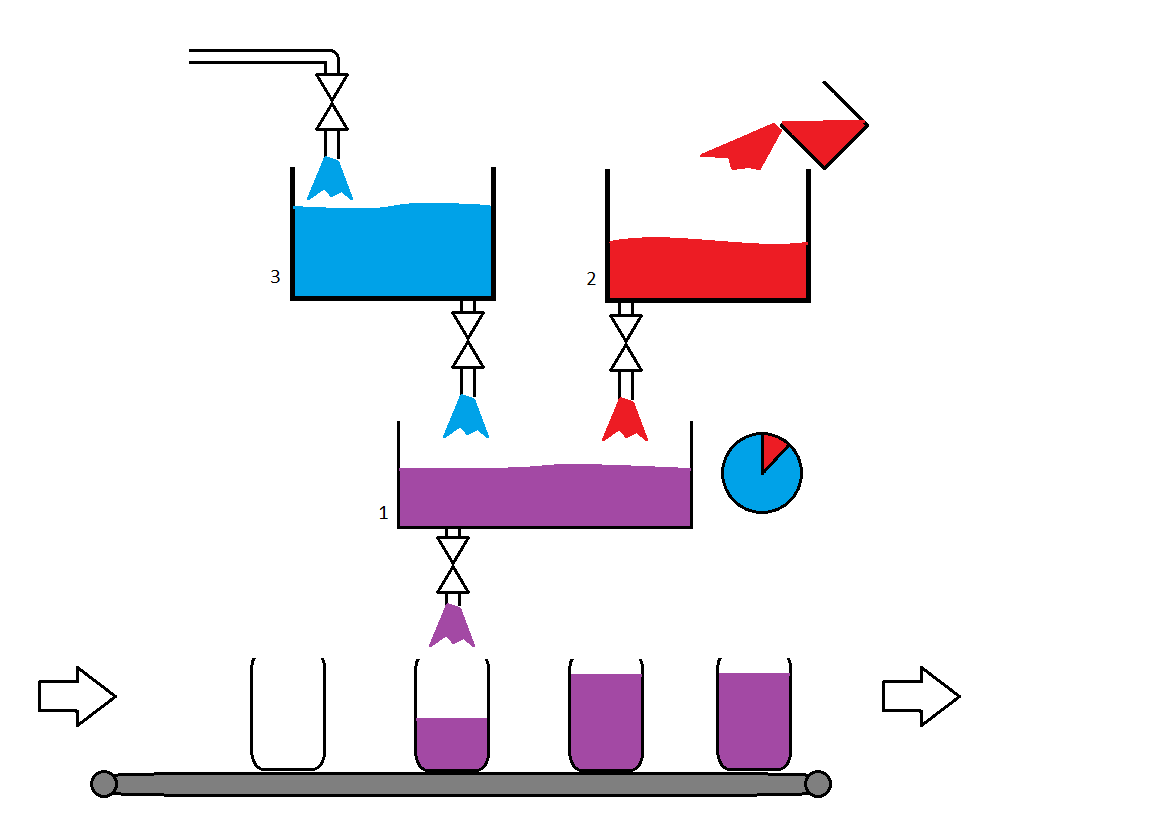
\includegraphics[scale = 0.4]{fig/Proces_schema.png}
	\caption{Schemat procesu.}
	\label{fig:Proces}
\end{figure}

\section{Regulatory}
\subsection{Regulacja poziomu wody w zbiorniku 3}
\indent Regulacja poziomu wody w zbiorniku 3 odbywa się poprzez regulator proporcjonalny sterujący stopniem otwarcia zaworu q4. Wartość sterowania wyliczana jest na podstawie uchybu pomiędzy wartością zadaną {h3\_SV} a wysokością poziomu wody w zbiorniku h3.
\begin{figure}[H]
	\centering
	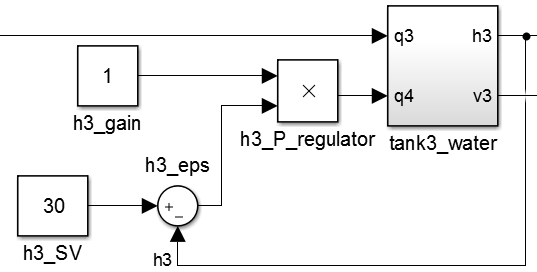
\includegraphics[scale = 0.4]{fig/h3_regulator.png}
	\caption{Schemat regulatora poziomu cieczy h3.}
	\label{fig:h3reg}
\end{figure}
\subsection{Regulacja poziomu koncentratu w zbiorniku 2}
\indent Regulacja poziomu koncentratu w zbiornkiu 2 odbywa się poprzez dolewanie dodatkowych porcji substancji przez pracownika po zgłoszeniu przez system komunikatu o niskim poziomie cieczy w zbiorniku. Aby zamodelować działanie pracownkia, który posiada pewną zwłokę w wykonywaniu działań oraz potrzebuje czasu na przemieszczenie się z dodatkową porcją koncentratu, użyto maszyny stanów. Określono czas reakcji pracowniak na komunikat systemowy, czas potrzebny do zabrania kolejnej porcji, oraz czas potrzebny na uzupełnienie koncentratu.
\subsection{Regulacja dawkowania wody i koncentratu do zbiornika mieszającego}
\indent Regulacja przepływu wody oraz koncentratu do zbiornika mieszającego odbywa się na podstawie pomiaru wysokości cieczy w zbiorniku 1 oraz na podstawie pomiaru stężenia koncentratu w gotowym produkcie. Regulacja odbywa się w taki sposób aby utrzymać zadany poziom w zbiuorniku oraz zadane stężenie gotowego produktu.
\subsection{Regulacja dawkowania gotowej mieszanki ze zbiornika mieszającego}
\indent Regulator odpowiedzialny za napełnianie pojemników gotową mieszanką działa poprzez maksymalne otwarcie wypływu ze zbiornika 1 aż do całkowitego napełnienia się naczynia. Po całkowitym napełnieniu zawór zostaje zamknięty aż do nadejścia kolejnego pojemnika do napełnienia.
